\documentclass{article}
\usepackage[a4paper,margin=1in,landscape]{geometry}
\usepackage[utf8]{inputenc}
\usepackage{amsmath}
\usepackage{amssymb}
\usepackage{tikz}
\usepackage{moresize}
\usepackage{graphicx}
\usepackage{enumitem}
\usepackage{minted}
\usepackage{fancyvrb}
\usepackage{xcolor}
\usepackage{hyperref}

\definecolor{lightlightgray}{rgb}{0.85,0.85,0.85}

\RecustomVerbatimCommand{\VerbatimInput}{VerbatimInput}%
{fontsize=\footnotesize,
 frame=lines,  
 framesep=2em, 
 rulecolor=\color{gray},
 label=\fbox{\color{black}output},
 labelposition=topline,
 commandchars=\|\(\), % escape character and argument delimiters for
                      % commands within the verbatim
 commentchar=*        % comment character
}

\usetikzlibrary{shapes, arrows, positioning}

\begin{document}
\noindent {\Large IFT-3655 : Modèles Stochastiques \\
Mathias La Rochelle}

\vspace{6cm}
\begin{center} \HUGE \textbf{DEVOIR 5}\end{center}

%%%% EXO 1
\newpage
%%%%%% Enonce
\noindent \textbf{1.} \textit{(10 points)} Pour chacun des deux exemples
de chaînes à 3 états à la page 65 de mes diapos, écrivez la matrice 
$\boldsymbol{P}$, puis calculer $\boldsymbol{\pi}$ et la matrice
$\boldsymbol{Q}$. On veut des valeurs numériques.

\vspace{.2cm}
\noindent En supposant que l'on part de 0, calculez la probabilité du chemin
$0\to 1\to 2\to 1\to 0$ à l'endroit et à l'envers (à reculons) dans 
chacun des deux cas. Vérifiez que ces probabilités sont en accord avec
le théorème de la page 73 des diapos. \\

%%%%%% Reponse
Pour la \textbf{première chaîne}, la matrice de transition $\boldsymbol{P}_1$ est
\begin{equation}
    \boldsymbol{P}_1=\begin{pmatrix}
        1/2 & 1/2 & 0 \\
        3/4 & 0 & 1/4 \\
        0 & 1/3 & 2/3
    \end{pmatrix}=\begin{pmatrix}
        0.50 & 0.50 & 0 \\
        0.75 & 0 & 0.25 \\
        0 & 0.33\overline{3} & 0.66\overline{6}
    \end{pmatrix}
\end{equation}

et les équations d'équilibre avec $\boldsymbol{\pi}\boldsymbol{P}=\boldsymbol{\pi}$ sont
\begin{gather}
    \pi_0=\frac{1}{2}\pi_0+\frac{3}{4}\pi_1 \\
    \pi_1=\frac{1}{2}\pi_0+\frac{1}{3}\pi_2 \\
    \pi_2=\frac{1}{4}\pi_1+\frac{2}{3}\pi_2 
\end{gather}

d'où on a
\[
    \pi_0=\frac{3}{2}\pi_1,\ \pi_2=\frac{3}{4}\pi_1
\]

et avec $\boldsymbol{\pi}\boldsymbol{1}^t=1$, on a
\begin{gather}
    \pi_0+\pi_1+\pi_2=1 \notag \\
    \frac{3}{2}\pi_1+\pi_1+\frac{3}{4}\pi_1=1 \notag \\
    \pi_1=\frac{4}{13}\approx0.3077
\end{gather}

puis,
\begin{gather}
    \pi_0=\frac{3}{2}\cdot\frac{4}{13}=\frac{6}{13}\approx0.4615 \\
    \pi_2=\frac{3}{4}\cdot\frac{4}{13}=\frac{3}{13}\approx0.2308
\end{gather}

Notre vecteur stationnaire pour la chaîne 1 est $\boldsymbol{\pi}_1=(0.4615\ 0.3077\ 0.2308)$. \\

\newpage
Pour calculer la matrice de transition $\boldsymbol{Q}_1$ de la chaîne à 
reculons, nous utilisons la condition $Q_{i,j}=(P_{j,i}\cdot\pi_j)/\pi_i$.
\begin{itemize}[left=1cm]
    \item $Q_{0,0}=\cfrac{1/2\cdot6/13}{6/13}=0.50$
    \item $Q_{0,1}=\cfrac{3/4\cdot4/13}{6/13}=0.50$
    \item $Q_{0,2}=\cfrac{0\cdot3/13}{6/13}=0$
    \item $Q_{1,0}=\cfrac{1/2\cdot6/13}{4/13}=0.75$
    \item $Q_{1,1}=\cfrac{0\cdot4/13}{4/13}=0$
    \item $Q_{1,2}=\cfrac{1/3\cdot3/13}{4/13}=0.25$
    \item $Q_{2,0}=\cfrac{0\cdot6/13}{3/13}=0$
    \item $Q_{2,1}=\cfrac{1/4\cdot4/13}{3/13}=0.33\overline{3}$
    \item $Q_{2,2}=\cfrac{2/3\cdot3/13}{3/13}=0.66\overline{6}$
\end{itemize}

La matrice de transition inverse $\boldsymbol{Q}_1$ est
\begin{equation}
    \boldsymbol{Q}_1=\begin{pmatrix}
        0.50 & 0.50 & 0 \\
        0.75 & 0 & 0.25 \\
        0 & 0.33\overline{3} & 0.66\overline{6}
    \end{pmatrix}
\end{equation}

\vspace{.5cm}
Pour la \textbf{deuxième chaîne}, la matrice de transition $\boldsymbol{P}_2$ est
\begin{equation}
    \boldsymbol{P}_2=\begin{pmatrix}
        0 & 1/5 & 4/5 \\
        4/5 & 1/5 & 0 \\
        0 & 4/5 & 1/5
    \end{pmatrix}=\begin{pmatrix}
        0 & 0.2 & 0.8 \\
        0.8 & 0.2 & 0 \\
        0 & 0.8 & 0.2
    \end{pmatrix}
\end{equation}

et les équations d'équilibre avec $\boldsymbol{\pi}\boldsymbol{P}=\boldsymbol{\pi}$ sont
\begin{gather}
    \pi_0=\frac{4}{5}\pi_1 \\
    \pi_1=\frac{1}{5}\pi_0+\frac{1}{5}\pi_1+\frac{4}{5}\pi_2 \\
    \pi_2=\frac{4}{5}\pi_0+\frac{1}{5}\pi_2 
\end{gather}

d'où on a
\[
    \pi_2=\frac{4}{5}\cdot\frac{4}{5}\pi_1+\frac{1}{5}\pi_2\to\pi_2=\frac{4}{5}\pi_1
\]

et avec $\boldsymbol{\pi}\boldsymbol{1}^t=1$, on a
\begin{gather}
    \pi_0+\pi_1+\pi_2=1 \notag \\
    \frac{4}{5}\pi_1+\pi_1+\frac{4}{5}\pi_1=1 \notag \\
    \pi_1=\frac{5}{13}\approx0.3846
\end{gather}

puis,
\begin{gather}
    \pi_0=\frac{4}{5}\cdot\frac{5}{13}=\frac{4}{13}\approx0.3077 \\
    \pi_2=\frac{4}{5}\cdot\frac{5}{13}=\frac{4}{13}\approx0.3077
\end{gather}

Notre vecteur stationnaire pour la chaîne 2 est $\boldsymbol{\pi}_2=(0.3077\ 0.3846\ 0.3077)$. \\

Pour calculer la matrice de transition $\boldsymbol{Q}_2$ de la chaîne à 
reculons, nous utilisons la même condition qu'avec la chaîne 1.
\begin{itemize}[left=1cm]
    \item $Q_{0,0}=\cfrac{0\cdot4/13}{4/13}=0$
    \item $Q_{0,1}=\cfrac{4/5\cdot5/13}{4/13}=1$
    \item $Q_{0,2}=\cfrac{0\cdot4/13}{4/13}=0$
    \item $Q_{1,0}=\cfrac{1/5\cdot4/13}{5/13}=0.16$
    \item $Q_{1,1}=\cfrac{1/5\cdot5/13}{5/13}=0.20$
    \item $Q_{1,2}=\cfrac{4/5\cdot4/13}{5/13}=0.64$
    \item $Q_{2,0}=\cfrac{4/5\cdot4/13}{4/13}=0.80$
    \item $Q_{2,1}=\cfrac{0\cdot5/13}{4/13}=0$
    \item $Q_{2,2}=\cfrac{1/5\cdot4/13}{4/13}=0.20$
\end{itemize}

La matrice de transition inverse $\boldsymbol{Q}_2$ est
\begin{equation}
    \boldsymbol{Q}_2=\begin{pmatrix}
        0 & 1 & 0 \\
        0.16 & 0.20 & 0.64 \\
        0.80 & 0 & 0.20
    \end{pmatrix}
\end{equation}

\vspace{.2cm}
Pour calculer la probabilité du chemin $0\to 1\to 2\to 1\to 0$, nous
utilisons $P$ à l'endroit et $Q$ à reculons. \\

Pour la \textbf{première chaîne}, on a à l'endroit
\begin{align}
    \mathbb{P}[X_1=1,X_2=2,X_3=1,X_4=0\mid X_0=0]&=\mathbb{P}[X_1=1\mid X_0=0]\cdot\mathbb{P}[X_2=2\mid X_1=1]\cdot\mathbb{P}[X_3=1\mid X_2=2]\cdot\mathbb{P}[X_4=0\mid X_3=1] \notag \\
    &=P_{1_{0,1}}\cdot P_{1_{1,2}}\cdot P_{1_{2,1}}\cdot P_{1_{1,0}} \notag \\
    &=0.5\cdot0.25\cdot0.33\overline{3}\cdot0.75 \notag \\
    &=0.03125 \notag
\end{align}

et à reculons
\begin{align}
    \mathbb{P}[X_1=1,X_2=2,X_3=1,X_4=0\mid X_0=0]&=Q_{1_{0,1}}\cdot Q_{1_{1,2}}\cdot Q_{1_{2,1}}\cdot Q_{1_{1,0}} \notag \\
    &=0.5\cdot0.25\cdot0.33\overline{3}\cdot0.75 \notag \\
    &=0.03125 \notag
\end{align}

Pour la \textbf{deuxième chaîne}, on a à l'endroit
\begin{align}
    \mathbb{P}[X_1=1,X_2=2,X_3=1,X_4=0\mid X_0=0]&=\mathbb{P}[X_1=1\mid X_0=0]\cdot\mathbb{P}[X_2=2\mid X_1=1]\cdot\mathbb{P}[X_3=1\mid X_2=2]\cdot\mathbb{P}[X_4=0\mid X_3=1] \notag \\
    &=P_{2_{0,1}}\cdot P_{2_{1,2}}\cdot P_{2_{2,1}}\cdot P_{2_{1,0}} \notag \\
    &=0.20\cdot0\cdot0.8\cdot0.8 \notag \\
    &=0 \notag
\end{align}

et à reculons
\begin{align}
    \mathbb{P}[X_1=1,X_2=2,X_3=1,X_4=0\mid X_0=0]&=Q_{2_{0,1}}\cdot Q_{2_{1,2}}\cdot Q_{2_{2,1}}\cdot Q_{2_{1,0}} \notag \\
    &=1\cdot0.64\cdot0\cdot0.16 \notag \\
    &=0 \notag
\end{align}

Pour la première chaîne, on remarque que la probabilité à l'endroit est égale la probabilité à l'envers. Donc la chaîne est
réversible. Pour la deuxième, il ne faut pas se référer aux probabilités calculées car une valeur nulle n'est pas représentatif 
de ce qui se passe. Sachant que nous avons certaines transitions qui ont valeurs de 0, regardons si leur transition inverse
est de 0 également, i.e. $P_{i,j}=0$ et $P_{j,i}=0$. On a $P_{2_{2,0}}=0$ mais $P_{2_{0,2}}=0.8$ alors la chaîne n'est
pas réversible.

\vspace{.1cm}
Petit supplément pour la première chaîne : la diagonale de 0 supporte bien le fait que la chaîne est réversible. C'est trivial.

%%%% EXO 2
\newpage
%%%%%% Enonce
\noindent \textbf{2.} \textit{(8 points)} Écrivez une preuve pour le 
théorème de la page 69 des diapos. (Ma solution fait 5 lignes.)

%%%%%% Reponse
\vspace{.2cm}
Supposons que $\boldsymbol{\pi}$ soit un vecteur de probabilités
stationnaires tel que $\sum_i\pi_i=1$ et que pour toute paire d'états
($i,j$), on ait l'égalité
\begin{equation}
    \pi_iP_{i,j}=\pi_jQ_{j,i}
\end{equation}

Par définition de la stationnarité, on a
\begin{equation}
    \pi_j=\sum_i\pi_iP_{i,j}
\end{equation}

et de même avec la chaîne inverse, on a
\begin{equation}
    \pi_i=\sum_j\pi_jQ_{j,i}
\end{equation}

En utilisant (18) (marche aussi avec (19)) et notre hypothèse posée 
plutôt, on retrouve
\[
    \pi_j=\sum_i\pi_iP_{i,j}=\sum_i\pi_jQ_{j,i}=\pi_j\sum_iQ_{j,i}
\]

et sachant que la somme des probabilités de transitions dans une matrice
stochastique est de 1, i.e. $\sum_iQ_{j,i}=1$, on a
\[
    \pi_j=\pi_j\sum_iQ_{j,i}=\pi_j
\]

Ceci démontre que les probabilités du vecteur stationnaire restent
inchangées pour la chaîne inverse.


%%%% EXO 3
\newpage
%%%%%% Enonce
\noindent \textbf{3.} \textit{(18 points)} On place $n$ processeurs 
dans une liste ordonnée. Lorsqu'une tâche arrive, le premier processeur 
dans la liste essaie de l'accomplir. S'il ne réussit pas, le second 
processeur essaie. S'il ne réussit pas, le processeur suivant essaie, 
et ainsi de suite. Dès qu'un processeur réussit, ou encore comme suit : 
si un processeur autre que le premier dans la liste réussit la tâche, 
on échange ce processeur avec celui qui le précède dans la liste. 
Ensuite une nouvelle tâche arrive et on si aucun processeur ne réussit, 
la tâche quitte le système, puis on réordonne les processeurs recommence. 
Supposons que les processeurs sont numérotés de 1 à $n$ et que le 
processeur $j$ réussit avec probabilité $p_j$ chaque fois qu'il essaie 
une tâche. \\

\noindent (a) Définissez une chaîne de Markov qui représente l'évolution 
de ce modèle. Il faut définir l'espace d'états, dire quelles sont les 
transitions possibles, et trouver leurs probabilités en fonction des 
$p_j$. Pour chaque transition possible, donnez aussi la probabilité de 
la transition inverse.

%%%%%% Reponse
\vspace{.5cm}
Chaque état de notre système est caractérisé par un vecteur $\boldsymbol{\sigma}_k$ qui est la $k$-ième configuration, i.e. 
$\boldsymbol{\sigma}_k=(\sigma_{k,1},\sigma_{k,2},...,\sigma_{k,n})$ où $\sigma_{k,i}$ est le $i$-ième processeur dans la 
configuration $k$. Par exemple, la configuration initiale serait dénotée comme $\boldsymbol{\sigma}_0=(\sigma_{0,1},...,\sigma_{0,n})$.
Le nombre de configurations possibles est le nombre de permutations des $n$ processeurs soit $n!$. \\

\noindent Dans ce système, une transition a lieu lorsqu'un processeur réussit. Alors disons nous avons le processeur $\sigma_{k,i}$
dans la position $i$ de la configuration $k$. S'il réussit, alors il prendra la position du processeur $\sigma_{k,i-1}$ et donc
cela signifie qu'on changera de configuration (état). Une deuxième type de transition est possible. Si aucun processeur de la
configuration $k$ réussit ou que le premier processeur de la configuration qui reçoit la tâche réussit, alors aucune permutation
entre un processeur et un autre se fera et donc on restera dans l'état courrant. \\

\noindent Décrivons désormais les probabilités de la matrice de transition $\boldsymbol{P}$. Il faut comprendre que la réussite
d'un processeur à la position $i$ dépend de l'échec des processeurs qui le précèdent. Donc disons pour quelconque configuration
$k$, le processeur 1 a $p_{\sigma_{k,1}}$ de réussir puis, $p_{\sigma_{k,2}}$ demande que le processeur 1 échoue avec probabilité
$1-p_{\sigma_{k,1}}$ puis, $p_{\sigma_{k,3}}$ demande que le processeur 1 et 2 échoue avec $1-p_{\sigma_{k,1}}$ et $1-p_{\sigma_{k,2}}$
et ainsi de suite.

\vspace{.3cm}
Donc, la probabilité de changer de configuration est
\[
    P_{\boldsymbol{\sigma}_i,\boldsymbol{\sigma}_j}=p_{\sigma_{i,t}}\cdot\prod_{m=1}^{t-1}\left(1-p_{\sigma_{i,m}}\right)
\]

\vspace{.2cm}
Quant à elle, la probabilité de rester dans la même configuration est
\[
    P_{\boldsymbol{\sigma}_i,\boldsymbol{\sigma}_i}=p_{\sigma_{i,1}}+\prod_{m=1}^{n}\left(1-p_{\sigma_{i,m}}\right)
\]

où $\boldsymbol{\sigma}_i=(\sigma_{i,1},...,\sigma_{i,t-1},\sigma_{i,t},...,\sigma_{i,n})$ et
$\boldsymbol{\sigma}_j=(\sigma_{j,1},...,\sigma_{j,t},\sigma_{j,t-1},...,\sigma_{j,n})$. 

\vspace{.2cm}
Pour la probabilité de la transition inverse d'un état à un autre, il faut que celui qui a été promu, à l'étape d'avant,
échoue à l'étape qui suit et que celui qui avait échoué avant réussit maintenant. En d'autres mots :
\[
    P_{{\boldsymbol{\sigma}_j,\boldsymbol{\sigma}_i}}=(1-p_{\sigma_{j,t}})\cdot p_{\sigma_{j,t-1}}\cdot\prod_{m=1}^{t-2}(1-p_{\sigma_{j,m}})
\]

\newpage
\noindent (b) Montrez que cette chaîne de Markov est réversible
et trouvez une formule pour les probabilités d'équilibre. Suggestion :
Trouvez un vecteur $\boldsymbol{\pi}$ qui est réversible pour la chaîne. \\


Quand on bouge un processeur $\sigma_{i,k}$ vers la gauche, on lui donne
une position plus favorable dans la file d'attente des processeurs donc 
qu'il aura plus de chances d'être choisies lors du traitement de la 
prochaine tâche. Cette tendance est quantifiée par 
$q_{\sigma_{i,t}}/p_{\sigma_{i,t}}$.
Inversement, quand on le bouge vers la droite, on lui
donne une position qui lui sera moins favorable et donc
$p_{\sigma_{j,t-1}}/q_{\sigma_{j,t-1}}$.

\vspace{.2cm}
Si la chaîne est réversible, alors elle satisfait l'équation
\begin{align}
    \pi_{\boldsymbol{\sigma}_i}P_{\boldsymbol{\sigma}_i,\boldsymbol{\sigma}_j}&=\pi_{\boldsymbol{\sigma}_j}P_{\boldsymbol{\sigma}_j,\boldsymbol{\sigma}_i} \\
    \pi_{\boldsymbol{\sigma}_i}&=\pi_{\boldsymbol{\sigma}_j}\frac{P_{\boldsymbol{\sigma}_j,\boldsymbol{\sigma}_i} }{P_{\boldsymbol{\sigma}_i,\boldsymbol{\sigma}_j}} \notag \\
    %\pi_{\boldsymbol{\sigma}_i}&=\pi_{\boldsymbol{\sigma}_j}\frac{p_{\sigma_{j,t-1}}/q_{\sigma_{j,t-1}}}{q_{\sigma_{i,t}}/p_{\sigma_{i,t}}} \notag \\
    \pi_{\boldsymbol{\sigma}_i}&=\pi_{\boldsymbol{\sigma}_j}\frac{(1-p_{\sigma_{j,t}})\cdot p_{\sigma_{j,t-1}}\cdot\prod_{m=1}^{t-2}(1-p_{\sigma_{j,m}})}{p_{\sigma_{i,t}}\cdot\prod_{m=1}^{t-1}\left(1-p_{\sigma_{i,m}}\right)} \notag \\
    \pi_{\boldsymbol{\sigma}_i}&=\pi_{\boldsymbol{\sigma}_j}\frac{(1-p_{\sigma_{j,t}})\cdot p_{\sigma_{j,t-1}}\cdot\prod_{m=1}^{t-2}(1-p_{\sigma_{j,m}})}{p_{\sigma_{i,t}}\cdot(1-p_{\sigma_{i,t-1}})\cdot\prod_{m=1}^{t-2}\left(1-p_{\sigma_{i,m}}\right)} \notag \\
    \pi_{\boldsymbol{\sigma}_i}&=\pi_{\boldsymbol{\sigma}_j}\frac{q_{\sigma_{j,t}}\cdot p_{\sigma_{j,t-1}}}{p_{\sigma_{j,t}}\cdot q_{\sigma_{j,t-1}}}
\end{align}

Petit exemple avec $n=3$. Disons que nous sommes dans la configuration $\boldsymbol{\sigma}_i=(\sigma_{i,2},\sigma_{i,3},\sigma_{i,1})$ 
et que nous voulons nous rendre à $\boldsymbol{\sigma}_0$. Il va donc falloir que le premier processeur bouge deux fois vers la gauche
et que les processeurs 2 et 3 bougent une fois vers la droite, i.e. $(\sigma_{i,2},\sigma_{i,3},\sigma_{i,1})\to(\sigma_{j,2},\sigma_{j,3},\sigma_{j,1})\to(\sigma_{k,2},\sigma_{k,3},\sigma_{k,1})$. 
Donc on va avoir la multiplication $(q_{\sigma_{i,1}}/p_{\sigma_{i,1}})^2\cdot p_{\sigma_{j,2}}/q_{\sigma_{j,2}}\cdot p_{\sigma_{k,3}}/q_{\sigma_{k,3}}$ 
et on termine avec $\boldsymbol{\sigma}_0=(\sigma_{0,1},\sigma_{0,2},\sigma_{0,3})$. Notre processeur $\sigma_{i,1}$ 
est parti de la position 3 et devait se rendre à la position 1 donc il a du faire $|1-\sigma_{i,1}|$ déplacement vers la droite.

\vspace{.2cm}
Ceci peut être généraliser tel qu'un processeur $\sigma_{i,t}$ doit bouger $|t-\sigma_{i,t}|$ fois avant 
d'arriver à la position $t$. La distribution stationnaire est satisfaite par
\begin{equation}
    \pi_{\boldsymbol{\sigma}_i}=\prod_{t=1}^n \left(\frac{q_{\sigma_{i,t}}}{p_{\sigma_{i,t}}}\right)^{t-\sigma_{i,t}}
\end{equation}

et donc notre chaîne est réversible.

\vspace{.5cm}
\noindent (c) Quelle est la permutation qui aura la plus grande 
probabilité à l'état d'équilibre ? Prouvez-le en utilisant la formule
trouvée en (b).

\vspace{.2cm}
Au final, la permutation qui aura la plus grande probabilité à l'état d'équilibre sera
la configuration des processeurs classés en ordre décroissant (donc $\sigma_{i,1}$ à la plus grande probabilité) des 
$n$ processeurs dans le vecteur des probabilités $\mathcal{P}$. On peut représenter cet état stationnaire comme 
\[
    \pi_{\boldsymbol{\sigma}} = \left( \sigma_{\max(\mathcal{P})},\sigma_{\max(\mathcal{P} \setminus \sigma_{\max(\mathcal{P})} )},...,\sigma_{\min(\mathcal{P})} \right)
\]

À noter qu'on laisse tomber le numéro de la configuration en indice puisqu'on parle d'une configuration spécifique.
Donc $\sigma_{t}$ dans $\pi_{\boldsymbol{\sigma}}$ est le $t$-ième meilleur processeur.

\vspace{.2cm}
Comme discuter plus tôt, quand le rapport $q_{\sigma_t}/p_{\sigma_t}$ devient plus petit, i.e. $q_{\sigma_t}/p_{\sigma_t} <\!\!< 1$,
c'est qu'il devient plus difficile d'avancer dans la file. Cela signifie que le processeur à la position $t$ est 
plus avancé que celui à la position $m$ pour $m>t$.

%%%% EXO 4
\newpage
%%%%%% Enonce 
\noindent \textbf{4.} \textit{(14 points)} Soit 
$\mathcal{G}=(\mathcal{V},\mathcal{A})$ une graphe connexe non
orienté ayant un nombre fini de sommets. un $k$-coloriage du graphe 
est un vecteur qui donne une couleur à chaque sommet du graphe, en 
utilisant au plus $k$ couleurs. Pour un graphe de $d$ sommets, il y
a $k^d$ possibilités. Un $k$-coloriage est dit \textit{admissible} s'il
n'y a pas deux sommets adjacents qui ont la même couleur. Pour un graphe
quelconque, trouver le plus petit $k$ pour lequel il existe un 
$k$-coloriage admissible, ou calculer le nombre de $k$-coloriages
admissibles, ou encore générer au hasard un $k$-coloriage selon la loi
uniforme sur l'ensemble $\mathcal{C}$ de tous les coloriages admissibles,
sont des problèmes connus comme très difficiles.

\vspace{.2cm}
\noindent Pour générer des $k$-coloriages approximativement selon la 
loi uniforme sur $\mathcal{C}$, pour un $k$ fixé, on peut penser à
utiliser MCMC. L'idée est de construire une chaîne de Markov dont l'état
est un élément de $\mathcal{C}$ et les probabilités d'états stationnaires
correspondent à la loi uniforme sur l'ensemble $\mathcal{C}$. On a vu
en classe (diapo 89) comment faire cela via l'échantillonage de Gibbs,
en ré-échantillonnant la couleur d'un seul sommet à chaque étape. \\

\noindent (a) Si $k$ est trop petit, il se peut qu'il n'existe pas de
$k$-coloriage admissible, ou bien encore qu'il en existe, mais que la 
chaîne construite via Gibbs ne soit pas irréductible sur $\mathcal{C}$,
de sorte qu'on ne puisse pas atteindre tous les $k$-coloriages 
admissibles à partir d'un $k$-coloriage initial. Pour voir cela,
considérez un graphe en triangle (3 sommets et 3 arêtes). Expliquez
ce qui se passe avec l'échantillonage de Gibbs si $k=2$, puis si
$k=3$, puis si $k=4$.

\vspace{.2cm}
\noindent Si $\Delta$ est le degré maximum d'un sommet du graphe, on
peut prouver que si $k\ge\Delta +2$, alors la chaîne construite par 
Gibbs est irréductible sur $\mathcal{C}$, et donc la loi stationnaire
est uniforme sur $\mathcal{C}$. Par contre l'inverse n'est peut-être
pas toujours vrai. \\

Posons les bases de la méthode d'échantillonage de Gibbs. Nous savons 
qu'une chaîne construite à partir de cette méthode est irréductible
si et seulement si tous les états admissibles de celle-ci peuvent 
atteindre n'importe quel état sur $\mathcal{C}$, i.e. l'ensemble qui 
contient toutes les configurations admissibles.

\vspace{.2cm}
\textbf{Processus général} :
\begin{enumerate}[left=1cm]
    \item On choisit une configuration initiale aléatoirement. 
    Dans notre cas, disons tous les sommets de 
    $\mathcal{G}=(\mathcal{V},\mathcal{A})$, où 
    $|\mathcal{V}(\mathcal{G}|$ est le nombre de sommets, sont blancs.
    \item Pour chaque sommet $v\in\mathcal{V}$ de la configuration,
    on efface sa couleur et on la remplace en ré-échantillonnant cette couleur
    conditionnellement aux couleurs des sommets adjacents dans le graphe. 
\end{enumerate}

\vspace{.1cm}
\textbf{Les trois différents cas} : 

\vspace{.3cm}
\underline{\textbf{\textit{Cas 1}}}

\vspace{.1cm}
Dans le cas où $k=2$, la chaîne de Markov construite par échantillonnage de 
Gibbs ne sera pas irréductible sur l'ensemble des 2-coloriages admissibles 
du triangle. Il n'existe aucun 2-coloriage admissible pour un triangle. Quel que 
soit le choix de couleurs pour deux sommets adjacents, le troisième sommet sera 
toujours adjacent à deux sommets de couleurs différentes. Si nous commençons avec 
une configuration initiale (par exemple, tous les sommets blancs), et que nous 
essayons d'appliquer l'échantillonnage de Gibbs, on a :
\begin{enumerate}[left=1cm]
    \item Le premier sommet choisi pourra changer de couleur (par exemple, devenir noir).
    \item Le deuxième sommet choisi devra rester blanc pour maintenir l'admissibilité.
    \item Le troisième sommet sera bloqué, car quelle que soit sa couleur, il sera 
            adjacent à un sommet de la même couleur.
\end{enumerate}

En conséquence, pour $k=2$, la chaîne n'est pas irréductible et ne peut pas explorer 
l'espace des coloriages admissibles, car cet espace est vide pour un triangle avec 
seulement deux couleurs disponibles.

\vspace{.3cm}
\underline{\textbf{\textit{Cas 2}}}

\vspace{.1cm}
Dans le cas où $k=3$, la chaîne de Markov construite par échantillonnage de Gibbs 
sera irréductible sur l'ensemble des 3-coloriages admissibles du triangle. 
\begin{itemize}[left=1cm]
    \item Il existe des 3-coloriages admissibles du triangle (en attribuant une couleur 
          différente à chaque sommet).
    \item À partir de n'importe quel 3-coloriage admissible, on peut atteindre tous les 
          autres en ré-échantillonnant successivement la couleur de chaque sommet. 
    \item À chaque étape, le sommet considéré aura toujours au moins une couleur disponible 
          différente de ses deux voisins.
    \item Ainsi, on peut passer d'un 3-coloriage admissible à n'importe quel autre en 
          un nombre fini d'étapes.
\end{itemize}

\vspace{.3cm}
\underline{\textbf{\textit{Cas 3}}}

\vspace{.1cm}
Dans le cas où $k=4$, la chaîne sera également irréductible sur l'ensemble des 4-coloriages 
admissibles, pour les mêmes raisons que dans le cas $k=3$. 
\begin{itemize}[left=1cm]
    \item Il y aura plus de flexibilité dans le choix des couleurs à chaque étape, puisqu'on 
          dispose d'une couleur supplémentaire.   
    \item Tous les 3-coloriages admissibles sont également des 4-coloriages admissibles.
    \item On pourra donc atteindre encore plus de configurations différentes.
\end{itemize} 

Dans les deux cas ($k=3$ et $k=4$), la chaîne est irréductible et permet d'explorer efficacement 
l'espace des coloriages admissibles, contrairement au cas $k=2$ où la chaîne était bloquée. 

\vspace{.5cm}
\noindent (b) Considérons le petit graphe ci-bas, repris de mes diapos.
Pour $k=3$, combien y a-t-il d'éléments dans $\mathcal{C}$ pour ce 
graphe ? Est-ce que Gibbs donne une chaîne irréductible sur 
$\mathcal{C}$ ? Mêmes questions pour $k=4$ et pour $k=5$.
\begin{figure}[h]
    \centering
    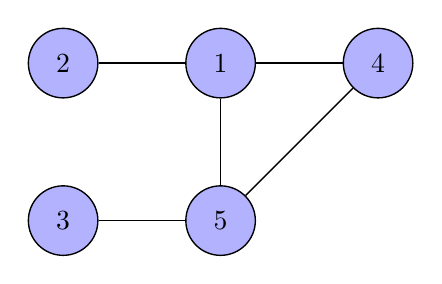
\begin{tikzpicture}[-,>=stealth', line width=0.5pt, node distance=2cm]
        \node [circle, draw, fill=blue!30, inner sep=6pt] (two) at (0, 2) {2};
        \node [circle, draw, fill=blue!30, inner sep=6pt] (one) at (2, 2) {1};
        \node [circle, draw, fill=blue!30, inner sep=6pt] (three) at (0, 0) {3};
        \node [circle, draw, fill=blue!30, inner sep=6pt] (five) at (2, 0) {5};
        \node [circle, draw, fill=blue!30, inner sep=6pt] (four) at (4, 2) {4};
        \path (two) edge (one);
        \path (three) edge (five);
        \path (one) edge (four);
        \path (one) edge (five);
        \path (five) edge (four);
    \end{tikzpicture}
\end{figure}

%%%%%% Reponse
Pour trouver le nombre d'éléments dans $\mathcal{C}$, soit
le nombre de configurations admissibles, on utilise un
algorithme glouton qui cherche parmi toutes les configurations
possibles, soit $k^{\mid\mathcal{V}(\mathcal{G})\mid}$, les
configurations qui respectent la règle qu'un sommet ne peut
avoir la même couleur que ses voisins.

\begin{minted}[bgcolor=lightlightgray, fontsize=\footnotesize, linenos]{python}
  
  from itertools import product

  G = {1: [2], 2: [3, 4], 3: [4], 4: [5], 5: []} # on pourrait faire G = {1: [2], 2: [1, 3, 4], 3: [2, 4], 4: [2, 3, 5], 5: [4]}
                                                 # mais ça prendrait plus de temps parce qu'on visiterait un sommet adjacent déjà visité
                                                 # dans depth_first_search()

  def generate_configs(k: int, G: dict) -> list:
      colors = [i for i in range(1, k + 1)] # on crée une séquence de couleurs (pour k = 3 on a [1,2,3], pour k = 4 on a [1,2,3,4], etc)
      return list(product(colors, repeat=len(G))) # on génère toutes les permutations distingables 
                                                  # source : https://www.hackerrank.com/challenges/itertools-product/problem

  def depth_first_search(config: tuple, G: dict) -> int:
      for i in range(len(config)):
          for v in G[i + 1]: # on regarde les sommets adjacents au sommet courant
              if config[v - 1] == config[i]: # si son sommet adjacent a la même couleur que lui, alors configuration non valide
                  return 0
      return 1

  ks = [3, 4, 5] # pour k = 3, puis k = 4, puis k = 5
  for k in ks:
      nb_configs = generate_configs(k, G)
      if len(nb_configs) == (k ** len(G)): # vérification qu'on a bien tous les configurations possibles
          nb_valid_config = 0
          for config in nb_configs:
              nb_valid_config += depth_first_search(config, G)
          print(f"Nombre de configurations admissibles pour un {k}-coloriage dans G : {nb_valid_config} sur {len(nb_configs)} configurations.")

\end{minted}

\VerbatimInput{output.txt}

En supposant que l'information donné à la question précédente est 
vraie, soit que si $k\ge\Delta+2$ où $\Delta$ est le degré maximum
parmi les sommets de $\mathcal{G}$, la chaîne construite par
Gibbs est irréductible sur $\mathcal{C}$, alors quand $k=3$, Gibbs 
ne donne pas une chaîne irréductible sur $\mathcal{C}$ car
$k\not\ge\Delta+2$ avec $\Delta=3$. Même chose avec $k=4$. Pour $k=5$,
on a bien une chaîne irréductible selon cette inégalité.

\newpage
Pour aller un peu plus loin pour $k=3$ puis $k=4$, dessinons ces configurations initiales : \\
\begin{figure}[h]
    \centering
    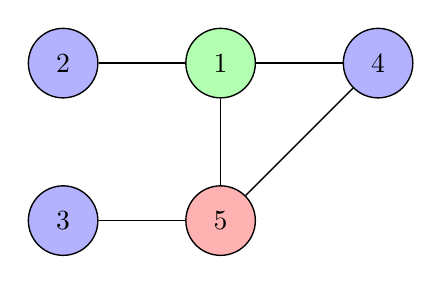
\begin{tikzpicture}[-,>=stealth', line width=0.5pt, node distance=2cm]
        \node [circle, draw, fill=blue!30, inner sep=6pt] (two) at (0, 2) {2};
        \node [circle, draw, fill=green!30, inner sep=6pt] (one) at (2, 2) {1};
        \node [circle, draw, fill=blue!30, inner sep=6pt] (three) at (0, 0) {3};
        \node [circle, draw, fill=red!30, inner sep=6pt] (five) at (2, 0) {5};
        \node [circle, draw, fill=blue!30, inner sep=6pt] (four) at (4, 2) {4};
        \path (two) edge (one);
        \path (three) edge (five);
        \path (one) edge (four);
        \path (one) edge (five);
        \path (five) edge (four);
    \end{tikzpicture}
    \caption{Pour $k=3$} 
\end{figure}

\vspace{.3cm}
\begin{figure}[h]
    \centering
    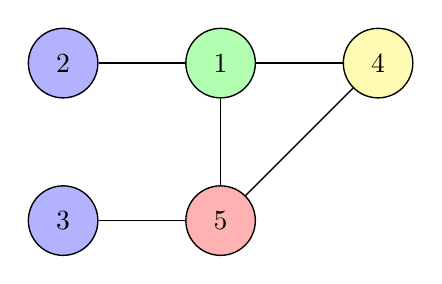
\begin{tikzpicture}[-,>=stealth', line width=0.5pt, node distance=2cm]
        \node [circle, draw, fill=blue!30, inner sep=6pt] (two) at (0, 2) {2};
        \node [circle, draw, fill=green!30, inner sep=6pt] (one) at (2, 2) {1};
        \node [circle, draw, fill=blue!30, inner sep=6pt] (three) at (0, 0) {3};
        \node [circle, draw, fill=red!30, inner sep=6pt] (five) at (2, 0) {5};
        \node [circle, draw, fill=yellow!30, inner sep=6pt] (four) at (4, 2) {4};
        \path (two) edge (one);
        \path (three) edge (five);
        \path (one) edge (four);
        \path (one) edge (five);
        \path (five) edge (four);
    \end{tikzpicture}
    \caption{Pour $k=4$}
\end{figure}

\vspace{.2cm}
Dans la figure 1, ni le sommet 1, ni le sommet 5 peuvent voir leur couleur changer sans
que cela entre en conflit avec la couleur des sommets qui leur sont adjacents. Puis, 
dans la figure 2, c'est le même cas avec le sommet 1 ; il peut ne prendre ni bleu, 
ni jaune, ni rouge. On conclut qu'à partir de ces sommets, il n'est jamais possible 
de se rendre à une autre configuration ce qui ne rejoint pas le concept d'irréductibilité.

\end{document}